\documentclass[12pt,a4paper]{article}
\usepackage{cmap} % Makes the PDF copiable. See http://tex.stackexchange.com/a/64198/25761
\usepackage[T1]{fontenc}
\usepackage[brazil]{babel}
\usepackage[utf8]{inputenc}
\usepackage{amsmath}
\usepackage{amsfonts}
\usepackage{amssymb}
\usepackage{amsthm}
\usepackage{textcomp} % \degree
\usepackage{gensymb} % \degree
\usepackage[usenames,svgnames,dvipsnames]{xcolor}
\usepackage{hyperref}
\usepackage{multicol}
\usepackage{graphicx}
\usepackage[margin=2cm]{geometry}

\hypersetup{
    colorlinks = true,
    allcolors = {blue}
}

\newcommand{\fixme}{{\color{red}(...)}}

\newcommand*\tipo{PROVA III}
\newcommand*\turma{TURMA B}
\newcommand*\disciplina{CDI0001}
\newcommand*\eu{Helder G. G. de Lima}
\newcommand*\data{28/05/2015}

\author{\eu}
\title{\tipo - \disciplina}
\date{\data}

\begin{document}
\thispagestyle{empty}
\newgeometry{margin=2cm,bottom=0.5cm}
\begin{center}

\includegraphics{udesc_joinville_cabecalho.pdf}
\\ Prof. \eu\footnote{
Este é um material de acesso livre distribuído sob os termos da licença \href{https://creativecommons.org/licenses/by-sa/4.0/deed.pt_BR}{Creative Commons BY-SA 4.0}.}

\noindent\begin{tabular}{l c c r}
  \textbf{\disciplina}
& \textbf{\tipo}
& \textbf{\data}
& \textbf{\turma}
\end{tabular}\vspace{-0.3cm}
\noindent\rule{17cm}{0.01cm}
\end{center}

\noindent Nome do aluno: \rule{14cm}{0.01cm}

%\section*{Instruções}
{\footnotesize
\begin{enumerate}
\renewcommand{\theenumi}{\Roman{enumi}}
\item Identifique-se em todas as folhas.
\item Mantenha o celular e os demais equipamentos eletrônicos desligados durante a prova.
\item Justifique cada resposta com cálculos ou argumentos baseados na teoria estudada.
\item Escolha \textsc{\textbf{uma}} das 6 questões para \textsc{\textbf{não}} fazer (ela não será corrigida): \rule{3cm}{0.01cm}
\end{enumerate}
}
\noindent\rule{17cm}{0.01cm}
%\section*{Questões}
\begin{enumerate}
\item Calcule os seguintes limites usando as regras de L'Hôpital, se possível:
\begin{multicols}{2}
\begin{enumerate}
\item (1,0 ponto) $\lim\limits_{x\to 0+} x^{\operatorname{sen}{(x)}}$
\item (1,0 ponto) $\lim\limits_{x\to -2} \dfrac{x^4+2x^3-2x^2-3x+2}{\ln{(x^2-3)}}$
\end{enumerate}
\end{multicols}

\item Utilize as regras de L'Hôpital para calcular os seguintes limites, se possível:
\begin{multicols}{2}
\begin{enumerate}
\item (1,0 ponto) $\lim\limits_{x\to 0} \dfrac{\operatorname{sen}{(3x)} - 3\operatorname{sen}{(x)}}{x-\operatorname{sen}{(x)}}$
\item (1,0 ponto) $\lim\limits_{x\to 0} \left(\dfrac{x+1}{x}-\dfrac{1}{\ln{(x+1)}}\right)$
\end{enumerate}
\end{multicols}

\item (2,0 pontos) Em relação à função $f(x): [-4,4] \to \mathbb{R}$ cujo gráfico está esboçado a seguir, responda (e justifique!):

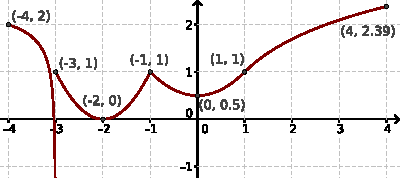
\includegraphics[width=8.0cm]{img/prova-3-tads-1-fig-1}

\begin{enumerate}
\item Em que ponto(s) ou intervalo(s) $f^\prime(x) < 0$, $f^\prime(x) > 0$, $f^\prime(x) = 0$ ou não existe $f^\prime(x)$?
\item Em que intervalo(s) $f^{\prime\prime}(x) < 0$? E em que intervalo(s) $f^{\prime\prime}(x) > 0$?
\item Quais os pontos de máximo, mínimo (relativos ou absolutos) e inflexão de $f(x)$?
\end{enumerate}

\item (2,0 pontos) Determine dois números cuja soma seja 15, tais que o seu produto seja o maior possível.
\item (2,0 pontos) Mostre que entre os retângulos que têm uma mesma área $A$, o quadrado é o que tem o menor perímetro.

\item Esboce os gráficos das seguintes funções, indicando (com justificativas!) os máximos, mínimos, intervalos de  (de)crescimento, concavidade e assintotas (se existirem):
\begin{multicols}{2}
\begin{enumerate}
\item (1,0 ponto) $f(x) = (x - 2) e^x$
\item (1,0 ponto) $g(x) = 3x^4 - 4x^3 + 1$
\end{enumerate}
\end{multicols}

\end{enumerate}

\begin{enumerate}
\renewcommand{\theenumi}{\alph{enumi}}%
\item

\includegraphics[width=16.0cm]{img/prova-3-tads-1-fig-2}
\vspace{2em}
\item

\includegraphics[width=16.0cm]{img/prova-3-tads-1-fig-2}
\end{enumerate}
%\newpage
%\restoregeometry
%\section*{Respostas e observações}
%
%\begin{enumerate}
%\item \fixme
%\end{enumerate}

\end{document}
